\section{Background}
\label{sec:bg}

In this section, we provide relevant details pertaining to the NEMD simulation in~\ref{sub:nemd}, 
key theoretical aspects of the active subspace methodology in~\ref{sub:as}, and provide a 
brief discussion on mathematical linkages between the total Sobol index, DGSMs, and the activity
scores (obtained from the active subspace) in~\ref{sub:scores}. These linkages could be exploited for the purpose of
global sensitivity analysis of the uncertain SW potential parameters in an efficient manner. 

\subsection{NEMD simulation}
\label{sub:nemd}

The NEMD simulations in this work were performed using the LAMMPS software~\cite{Plimpton:2007}.
Specifically, the simulations were performed for a Si bar of length, $L$, subjected to a temperature gradient, 
$\left(\frac{dT}{dz}\right)$. The temperature gradient was applied by means of Langevin thermostats located
at $L/4$ and $3L/4$. Schematic illustration of the set-up and the arrangement of atoms is provided below in 
Figure~\ref{fig:setup}.
%
\begin{figure}[htbp]
\begin{center}
\begin{tabular}{cc}
  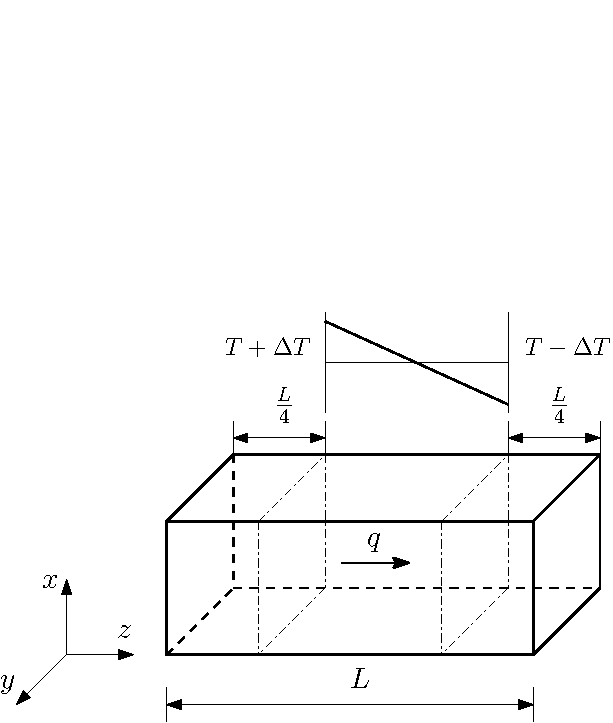
\includegraphics[width=0.48\textwidth]{./Figures/schematic}
  &
  \hspace{3mm}
  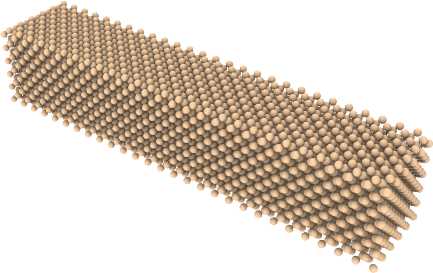
\includegraphics[width=0.40\textwidth]{./Figures/Sibar_05}
  \\ (a) & (b)
  \end{tabular}
\caption{(a) Schematic illustration of the simulation set-up for estimating the thermal conductivity of a Si bar of
length, $L$, subjected to a temperature gradient, $\left(\frac{4\Delta T}{L}\right)$, (b) 
Initial configuration of Si atoms in the bar.}
\label{fig:setup}
\end{center}
\end{figure}
%
The heat flux between the thermostats at the end of the simulation ($q$, W/m$^2$) is recorded to compute the
thermal conductivity of the Si bar using Fourier's law:
%
\be
 \kappa = \frac{q}{\left|\frac{dT}{dz}\right|} 
\ee
%
where $\left|\frac{dT}{dz}\right|$ denotes the magnitude of the applied thermal gradient. In Table~\ref{tab:input},
we provide the set of inputs used to perform the NEMD simulation. Note that the simulation run length, width, 
and height were selected to minimize temperature fluctuations during the different stages of the simulation while
ensuring a reasonable computational effort. 
%
\begin{table}[htbp]
\centering
\ra{1.3}
\begin{tabular}{@{}cc@{}}\toprule
Lattice Constant, $a$ ($\angstrom$) & 5.43 \\ 
Width, Height ($\angstrom$) & 22$a$ \\
$\Delta t$  (ps) & 0.0005 \\ 
Simulation Run Length (ps) & 320 \\ 
Boundary Condition & Periodic \\ 
Lattice Structure & Diamond \\
Inter-atomic Potential & Stillinger-Weber \\ 
\bottomrule
\end{tabular}
\caption{The set of LAMMPS inputs for performing the NEMD simulation of a Si bar illustrated in Figure~\ref{fig:setup}.}
\label{tab:input}
\end{table}
 
As illustrated in the following flow diagram, there are four stages involved in the NEMD simulation: 
NPT, NVT, NVE (I), and
NVE (II); NPT, NVT and NVE are thermodynamic ensembles used commonly in NEMD simulations. We have used
(I) and (II) here to distinguish between the two NVE ensembles. 
%
\begin{center}

NPT \hspace{5mm} $\rightarrow$ \hspace{5mm} NVT \hspace{5mm} $\rightarrow$ \hspace{5mm} NVE (I) \hspace{5mm}
$\rightarrow$ \hspace{5mm} NVE (II)
\\ \vspace{1mm}
\tiny [Relax the system]~[Equilibrate system to 300 K] \hspace{1mm} [Equilibrate thermostats] \hspace{4mm}
 [Generate Data]
\\ \vspace{1mm}

\tiny{N: Number of Atoms~~~P: Pressure~~~V: Volume~~~T: Temperature~~~E: Energy}
\end{center}
%
Initially, our NEMD simulation set-up did not comprise an NPT ensemble. However,
since computing the active subspace involves pseudorandom sampling of the marginal distributions
of the SW potential parameters, it was observed that the structural integrity of the Si bar was lost for
certain set of parameter values. To circumvent this challenge, an NPT ensemble was run
(for a sufficiently long time), prior to the NVT ensemble to ensure that the system relaxes to a 
steady value of the bar length as discussed in~\cite{Vohra:2018a}.
During the NVT stage, the system is equilibrated to a specific bulk temperature at which the thermal
conductivity of the bar is to be estimated. The NVE (I) stage involves equilibration of the thermostats
at specified temperatures. Lastly, during the NVE (II) stage, the trajectory of individual atoms during
simulation is recorded.

\subsection{Active Subspace}
\label{sub:as}

As mentioned earlier in section~\ref{sec:intro}, the active subspace is a low-dimensional space in the
input domain that sufficiently captures the variability in the QoI~\cite{Constantine:2015}.
Uncertain model inputs, $\bm{\theta}$, are parameterized as canonical random variables, 
$\bm{\xi}\in\Omega\in\mathbb{R}^{N_\theta}$, where $N_{\theta}$ denotes the number of uncertain inputs. 
Pseudorandom samples are generated according the joint probability distribution of $\xi_i$'s ($\pi_\vec\xi$).
The samples are then projected back to the physical space to evaluate the model output, $G$. The
active subspace is spanned by the dominant eigenvectors of a symmetric and positive semidefinite matrix,
$\mat{C}$:
%
\be
\mat{C} = \int_\Omega (\nabla_{\vec{\xi}}G)(\nabla_{\vec{\xi}}G)^\top dP_\vec\xi, 
\label{eq:C}
\ee
%  
where $dP_\vec\xi$ = $\pi_\vec\xi d\vec\xi$. Note that $G$ is assumed to differentiable in the considered
input domain. Additionally, $G$ and its partial derivatives in~\eqref{eq:C} are assumed to be L-2 
integrable. Consider the eigenvalue decomposition of $\mat{C}$:
%
\be
\mat{C} = \mat{W}\mat{\Lambda}\mat{W}^\top.
\ee
%
where $\mat{\Lambda}$ = diag($\lambda_1,\ldots,\lambda_\Nt$) with $\lambda_i$'s sorted in
descending order:
\[
     \lambda_1 \geq \lambda_2 \geq \cdots \geq \lambda_\Nt \geq 0.
\] 
%
The matrix, $\mat{W}$ comprises orthonormal eigenvectors as its columns. The eigenpairs are partitioned
about the $p^{th}$ eigenvalue such that, \scalebox{1.25}{$\left(\frac{\lambda_p}{\lambda_{p+1}}\right)$}$\gg 1$
as follows:
%
\be
 \mat{W} = [\mat{W}_1~\mat{W}_2],~~\mat{\Lambda} = \begin{bmatrix}\mat{\Lambda}_1 & \\  &
  \mat{\Lambda}_2. 
\end{bmatrix}
\ee
%
The column space of $\mat{W}_1$ constitutes the dominant eigenspace of $\mat{C}$, regarded as the
active subspace, and $\mat{\Lambda}_1$ is the corresponding diagonal matrix with 
$\{\lambda_1,\ldots,\lambda_p\}$ as its entries. Dimension reduction is accomplished by transforming the
model output, $G(\vec\xi)$ (a function of $\Nt$ independent inputs) into $\mathcal{Y}(\vec\eta)$, a
function of $p$ independent inputs, where $\vec\eta$ = $\mat{W}_1^\top \vec\xi\in\mathbb{R}^p$, 
is referred to as the set of \textit{active variables}. Computational effort associated with UQ
is hence reduced by means of dimension reduction. However, to further decrease computational effort,
we approximate $\mathcal{Y}$ using a surrogate, $\tilde{\mathcal{Y}}$, constructed using the sequence of steps
provided in~\cite{Constantine:2015} (chapter 4), and outlined below in Algorithm~\ref{alg:surr}.
\bigskip
\begin{breakablealgorithm}
\renewcommand{\algorithmicrequire}{\textbf{Input:}}
\renewcommand{\algorithmicensure}{\textbf{Output:}}
  \caption{For constructing the surrogate model, $\tilde{\mathcal{Y}}(\mat{W}_1^\top\vec\xi)$}
  \begin{algorithmic}[1]
	\Procedure{Surrogate Model, $\tilde{\mathcal{Y}}$}{} 
	  \State Consider $N$ available data points in the full space, $(\vec\xi_i,G(\vec\xi_i))$, $i~=~1,\ldots,N$
	  \State For each $\vec\xi_i$, compute $\vec\eta_i$ = $\mat{W}_1^\top\vec\xi_i$ 
          (Note: $\mathcal{Y}(\vec{\eta}_i)$ $\approx$ $G(\vec{\xi}_i)$)
	  \State Fit a regression surface, $\tilde{\mathcal{Y}}$ to approximate $\mathcal{Y}$ using the data
                 points, $(\vec\xi_i,\mathcal{Y}(\vec\eta_i))$
	  \State Note that the overall approximation is: $G(\vec{\xi})$ $\approx$
                 $\tilde{\mathcal{Y}}(\mat{W}_1^\top\vec{\xi})$ 
	\EndProcedure
  \end{algorithmic}
  \label{alg:surr}
\end{breakablealgorithm}
\bigskip

In practice, the matrix, $\mat{C}$ is numerically approximated using model gradient estimates at random samples
in the input space as follows:
 %
 \be
 \mat{C}\approx \hat{\mat{C}} = \frac{1}{N}\sum\limits_{i=1}^{N} 
 (\nabla_{\vec{\xi}}G(\vec{\xi}_i))(\nabla_{\vec{\xi}}G(\vec{\xi}_i))^\top
 = \hat{\mat{W}}\hat{\mat{\Lambda}}\hat{\mat{W}}^\top.
\label{eq:chat}
 \ee
 %
Hence, the computational effort required for constructing $\hat{\mat{C}}$ scales with the number of samples, $N$.
To avoid excessive number of model evaluations and hence optimize the computational effort, the regression-based
approach for gradient estimation is employed to compute the active subspace
in an iterative manner as discussed in~\ref{sub:gradient} and~\ref{sub:subspace}. Furthermore, the
active subspace could be exploited to perform a global sensitivity analysis (GSA) of the SW parameters as
discussed in~\ref{sub:scores}.



































